\subsection{Math problem-solving: partially-relational sequence-to-sequence tasks}\label{ssec:experiments_math}

The object-sorting experiments in the previous section are ``purely relational'' in the sense that the set of pairwise $\prec$ relations is a sufficient statistic for solving the task.
%  (i.e., the target sequence is conditionally independent of the input sequence given the relations)
In a general sequence-to-sequence task, however, there may not be a relation which is a sufficient statistic. Nonetheless, relational reasoning may still be crucial for solving the task, and the enhanced relational reasoning capabilities of the Abstractor may enable performance improvements. The ``partially-relational'' architectures described in~\Cref{sec:abstractor_architectures} enable a branch of the model to focus on relational reasoning while maintaining a connection to object-level attributes. In this section, we evaluate an Abstractor model (using architecture (d) of~\Cref{fig:abstractor_architectures}) on a set of math problem-solving tasks based on the dataset proposed by~\citet{saxtonAnalyzingMathematicalReasoning2019}.

\begin{figure}
    \vskip-10pt
    \begin{center}
    \begin{small}
    \begin{tabular}{cc}
        \begin{tabular}{l}
        Task: \texttt{polynomials\_\_expand}\\
        Question: \texttt{Expand (2*x + 3)*(x - 1).}\\
        Answer: \texttt{2*x**2 + x - 3}
        \end{tabular}
        &
        \begin{tabular}{l}
        Task: \texttt{algebra\_\_linear\_1d}\\
        Question: \texttt{Solve for z: 5*z + 2 = 9.}\\
        Answer: \texttt{7/5}
        \end{tabular}
    \end{tabular}
    \end{small}
    \end{center}
    \vskip-10pt
    \caption{Examples of input/target sequences from the math problem-solving dataset.}\label{fig:math_dataset}
    \vskip-15pt
\end{figure}

The dataset consists of several math problem-solving tasks, with each task having a set of question-answer pairs. The tasks include solving equations, expanding products of polynomials, differentiating functions, predicting the next term in a sequence, etc. A sample of question-answer pairs is displayed in~\Cref{fig:math_dataset}. The overall dataset contains $2 \times 10^6$ training examples and $10^4$ validation examples per task. Questions have a maximum length of 160 characters and answers have a maximum length of 30 characters. We use character-level encoding with a common alphabet of size $95$ (including upper/lower case characters, digits, punctuation, and special start/end/pad tokens). %Each question and answer is tokenized and padded with the null character.

We compare an Abstractor model using architecture (d) in~\Cref{fig:abstractor_architectures} to a standard Transformer. We evaluate an Abstractor with positional symbols and an Abstractor with symbolic attention (see~\Cref{ssec:symbol_assignment}). Since the Abstractor-based models with architecture (d) have an Abstractor module in addition to an Encoder and Decoder, we compare against two versions of the Transformer in order to control for parameter count. In the first, the Encoder/Decoder have identical hyperparameters to the Abstractor model. In the second, we increase the model dimension and hidden layer size of the feedforward network such that the overall parameter count is approximately the same as for the Abstractor model. We refer to the first model as ``Transformer'' and the second as ``Transformer+'' in the figures. %We train on modestly sized models. 
The precise architectural details and hyperparameters are described in~\Cref{sec:experimental_details}.

% \begin{wrapfigure}{R}{0.5\textwidth}
%     \centering
%     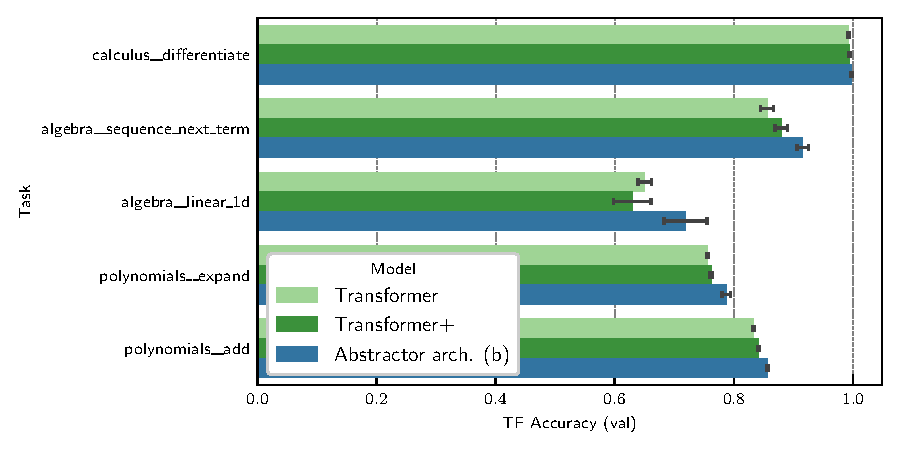
\includegraphics[width=0.5\textwidth]{figures/experiments/math_metrics.pdf}
%     \caption{\footnotesize End-of-training teacher-forcing accuracy.}\label{fig:math_metrics}
% \end{wrapfigure}

We evaluate the three models on five subtasks: differentiating functions (calculus); predicting the next term in a sequence (algebra); solving a linear equation (algebra); expanding polynomials; and adding polynomials. For each, we train on the training split and track the teacher-forcing accuracy (excluding null characters) on the validation split. For each pair of model and task, we repeat the experiment five times and report error bars as twice the standard error of the mean.

\begin{figure}[t]
    % \vskip-15pt
    \centering
    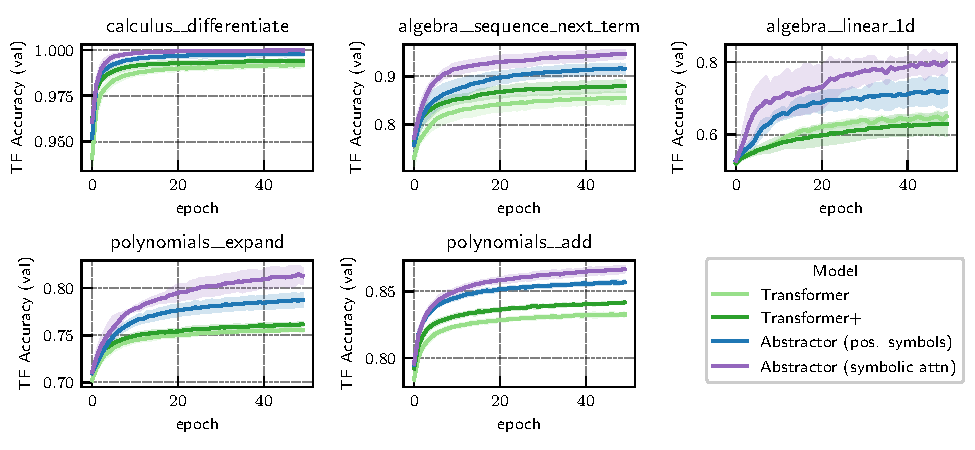
\includegraphics[width=\textwidth]{figures/experiments/math_training_curves.pdf}
    \vskip-10pt
    \caption{Training curves comparing an Abstractor-based architecture to a standard Transformer on mathematics problem-solving tasks.}\label{fig:math_training_curves}
    \vskip -15pt
\end{figure}

% \Cref{fig:math_metrics} shows the end-of-training teacher-forcing accuracy on the validation split for each task.~
\Cref{fig:math_training_curves} shows the validation teacher-forcing accuracy during the course of training, which we use as a proxy for sample-efficiency. We observe an improvement in accuracy compared to both `Transformer' and `Transformer+' across all tasks. The larger Transformer tends to perform better than the smaller Transformer, but the Abstractor-based model consistently outperforms both, with the symbolic attention mechanism showing the greatest improvement. This indicates that the performance improvement stems from the architectural modification and inductive bias. We conjecture that a ``partially-relational'' Abstractor architecture (e.g., architecture (d)) implements two branches of information-processing. The Encoder performs more general-purpose processing of the input sequence, while the Abstractor performs more specialized relational processing. The Decoder then has access to both representations, enabling it to perform the task more effectively.
